\srsfuncion{Consultar inventario}
	Esta función debe mostrar al usuario la lista completa de los items del inventario de la empresa.
		
	\begin{enumerate}
		\item \textit{Prioridad}: alta.
		\item \textit{Entradas}
			\begin{enumerate}
				\item Los items del inventario se mostrarán ordenados por defecto por orden alfabético, pero podrán ordenarse según: fecha de entrada en almacén, cantidad de items, destino de uso (oficina, mecánica, edificios, aeronáutico\ldots) y valor de adquisición.
			\end{enumerate}
		\item \textit{Flujo de operaciones}
			\begin{enumerate}
				\item Se muestra por pantalla una tabla con la lista de items disponibles en el inventario ordenada por orden alfabético. Se da la opción al usuario de ordenarla siguiendo los criterios anteriormente mencionados, cada uno de los cuales aparece en la parte superior de la tabla.																				\end{enumerate}
		\item \textit{Respuesta a situaciones no previstas}
			\begin{enumerate}
				\item Si no se puede acceder a la base de datos del inventario: se muestra por pantalla un mensaje para que el usuario se ponga en contacto con el personal técnico de la empresa y le manifieste el error, disculparse por las molestias y dar las gracias por el aviso.
				\item Si no se ha podido ordenar en orden alfabético: mostrar la información desordenada.
			\end{enumerate}
	\end{enumerate}
	
	\label{fun:ConsulInv}
	\begin{figure}[ht]\centering
	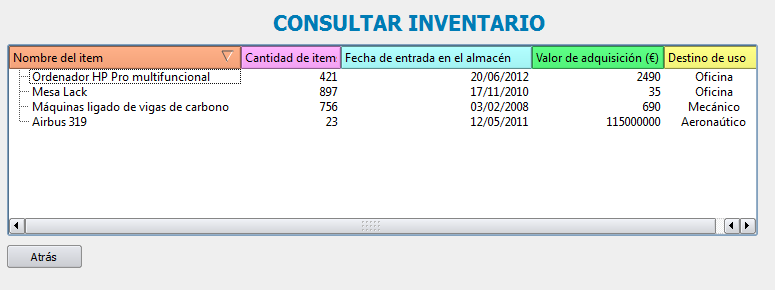
\includegraphics[scale=.6]{imagenes/consultarInventarioImagen.png}
	\caption{Pantalla aproximada de la consulta de inventario}
\end{figure}

								
